\section{Experiments}
\seclabel{experiments}

\subsection{Dataset}
To study the convergence rate with orders of magnitude of previous grasp data we create a dataset of tens of thousands of 3D CAD models.
We aggregated data from the laser scanned datasets Amazon Picking Challenge~\cite{}, BigBIRD~\cite{}, KIT~\cite{}, and YCB~\cite{}, as well as the synthetic datasets 3DNet~\cite{wohlkinger20123dnet} and the SHREC 2014 large-scale retrieval dataset~\cite{}.
To preprocess the data for grasping we set the frame of reference for each object to the the principal components of the vertices of each mesh, set the object center-of-mass as the center of a bounding box around the reoriented vertices, removed unreferenced and invalid vertices, rescaled each synthetic mesh such that its smallest principal direction fit within a PR2 gripper, and converted the mesh to a signed distance field.
We reserved the YCB dataset as a test set, and used subsets of the remaining data to train hyperparameters and to seed the CCBPs for convergence experiments on the test dataset.

\subsection{System}
To handle the scale of the experiments, we developed a Cloud-based software library on top of Google Cloud services.
We used Google Cloud Storage (GCS) to store the mesh models and to sample and evaluate 250 grasps per object.
Each model is stored in .OBJ format and the average size is roughly 0.5MB.
We used Google Compute Engine to distribute trials of MAB algorithms across objects, reducing the runtime of our large-scale experiments.
Our master analysis script can launch up to 600 GCE single core instances, each running Ubuntu 12.04.
When an instance is launched, we mount DexNet via a persistent disk containing a particular set of objects and grasps.
Each instance pulls our latest code from Github, runs a single python experiment script configured in a YAML file, compresses the results in an output directory, and uploads the results to GCS.
After all instances complete, the master script turns off all instances, unmounts all disks, downloads the results from each instance, and sends the user a notification email.
The results can be optionally analyzed by the master script.

\subsection{Rate of Convergence}
\TODO{Replace with final versions. The current results are preliminary}

Preliminary experiments suggest that using CCBPs with prior data from DexNet reduces the number of samples for MAB algorithms to converge to a grasp with high probablity of force closure $P_F$ under uncertainty in object pose, gripper pose, and friction coefficient.
~\figref{local-mab} shows the normalized $P_F$ (the ratio of the $P_F$ for the sampled grasp to the $P_F$ in the candidate grasp set) versus iteration averaged over 20 trials for a cereal box and flower pot.
The plot compares Thompson sampling, a MAB algorithm, without correlations to Thompson sampling using the CCBP model of local grasp similiarity (no prior data).
We see that the CCBP model outperforms the uncorrelated model by approximately 10$\times$ for the cereal box but has comparable performance to Thompson sampling on the flower pot.
Iniitial reuslts suggest that performance on the flower pot is poorer because it has very few similar grasps according to our similarity metric.

\begin{figure}[t!]
\centering
	\begin{subfigure}[b]{0.5\textwidth}
        \centering
        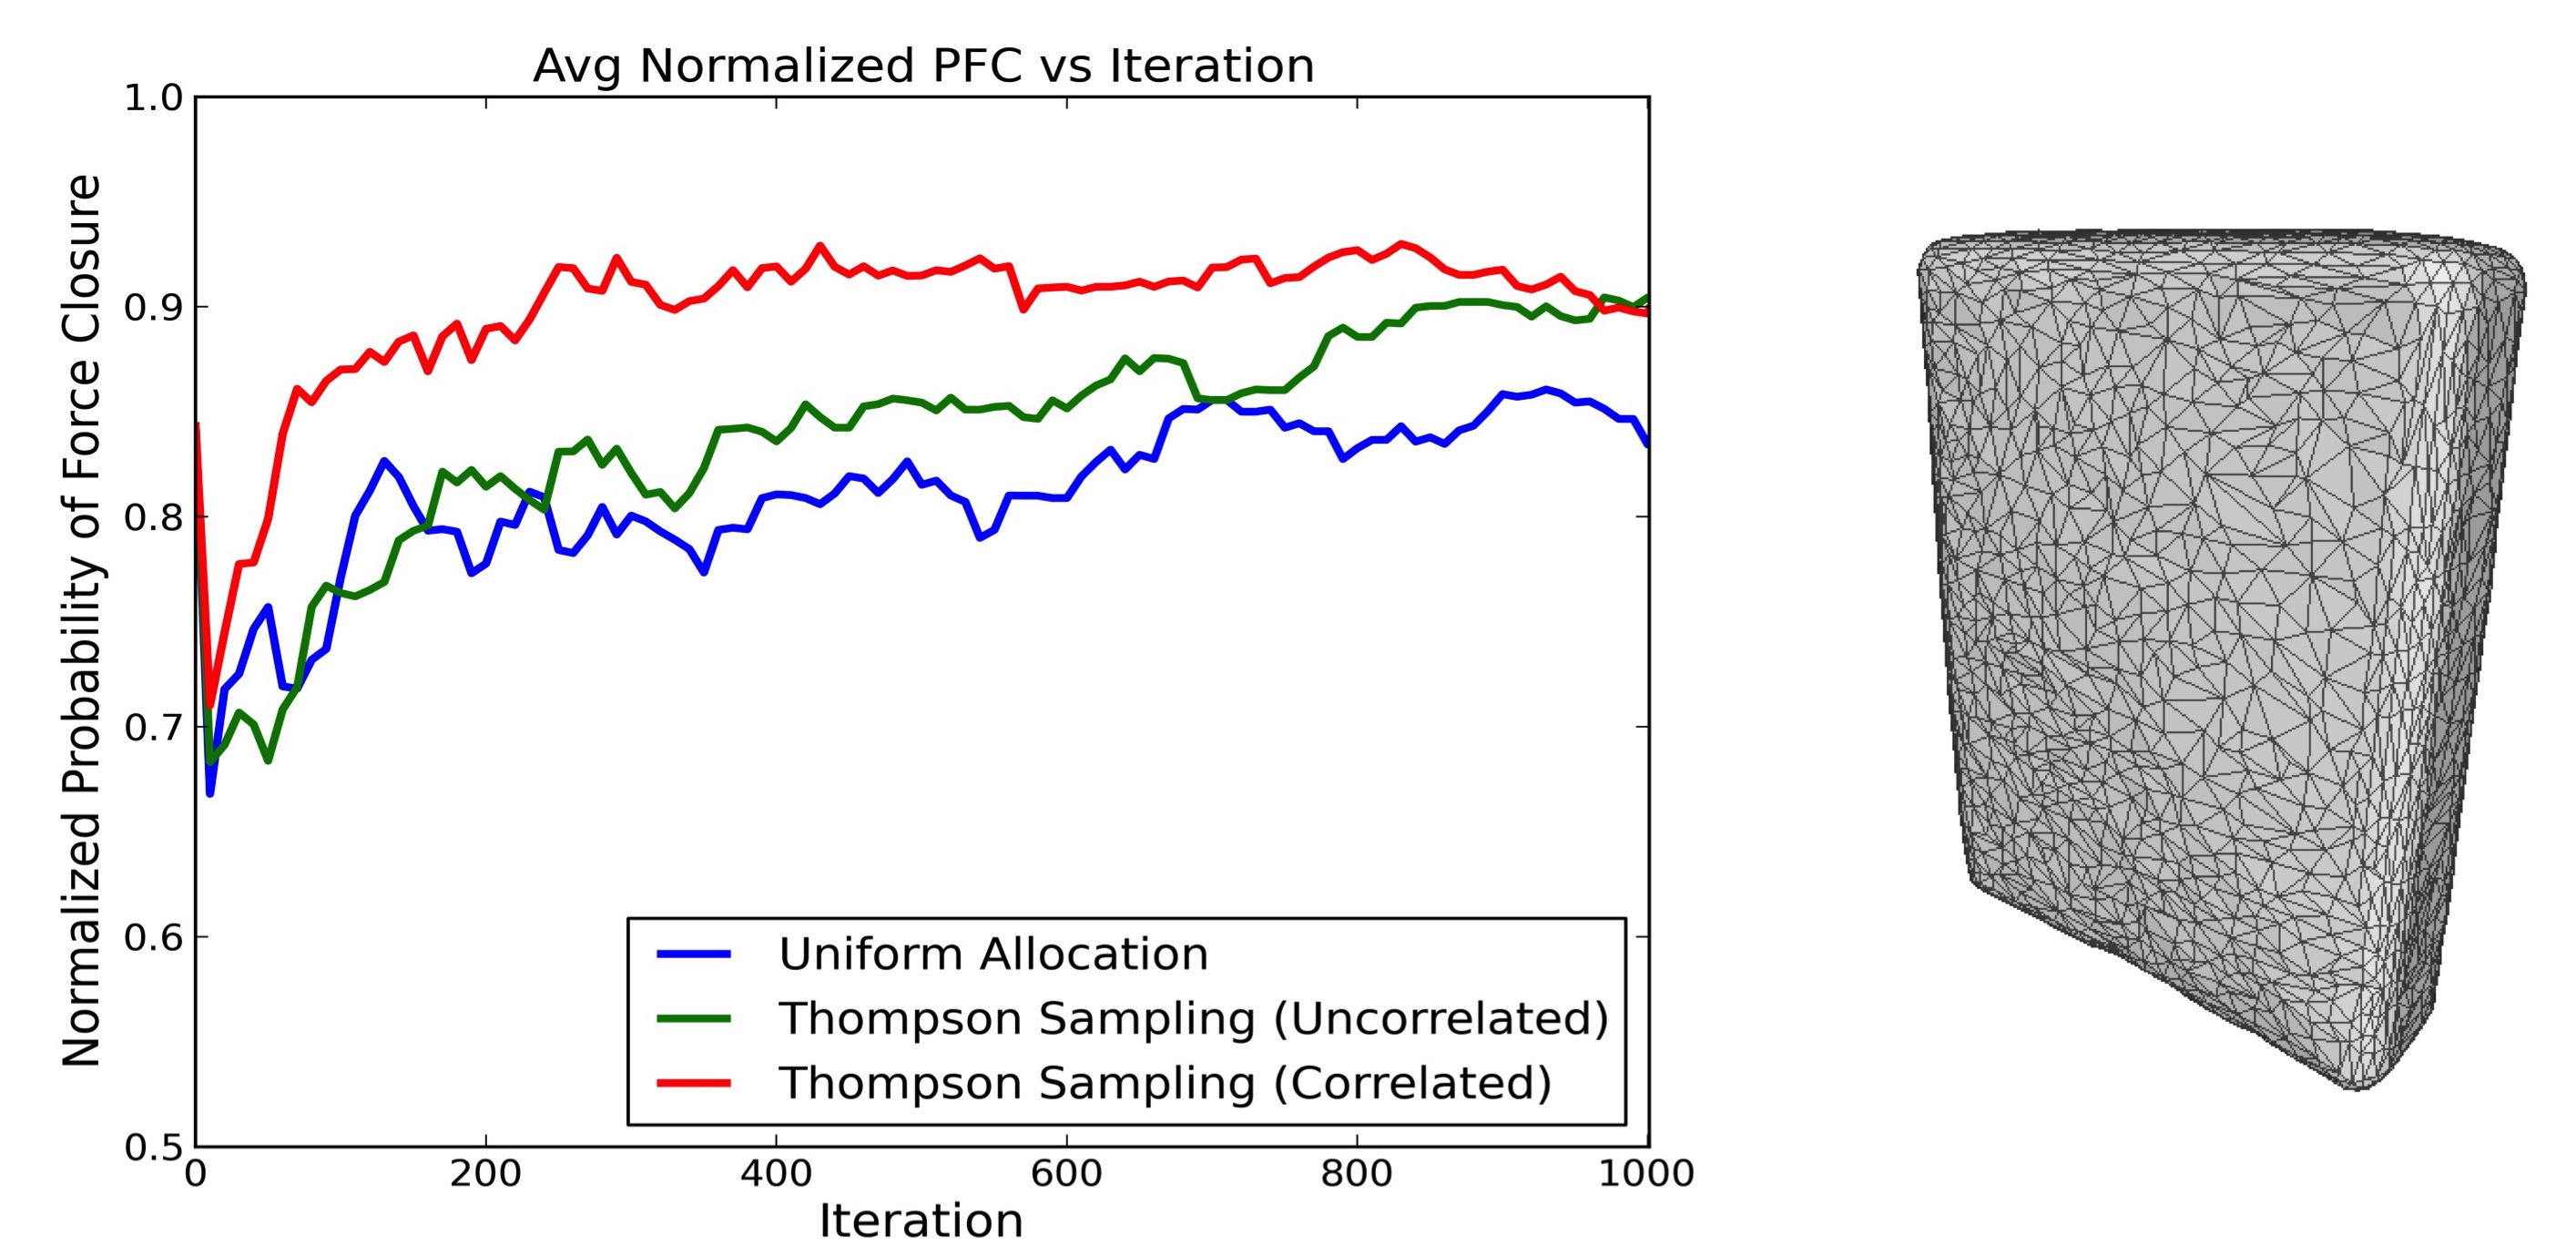
\includegraphics[scale=0.08]{figures/box_avg_reward_w_model.jpg}
        \caption{Normalized $P_F$ on a cereal box with 250 candidate grasps.}
    \end{subfigure}
    \begin{subfigure}[b]{0.5\textwidth}
        \centering
        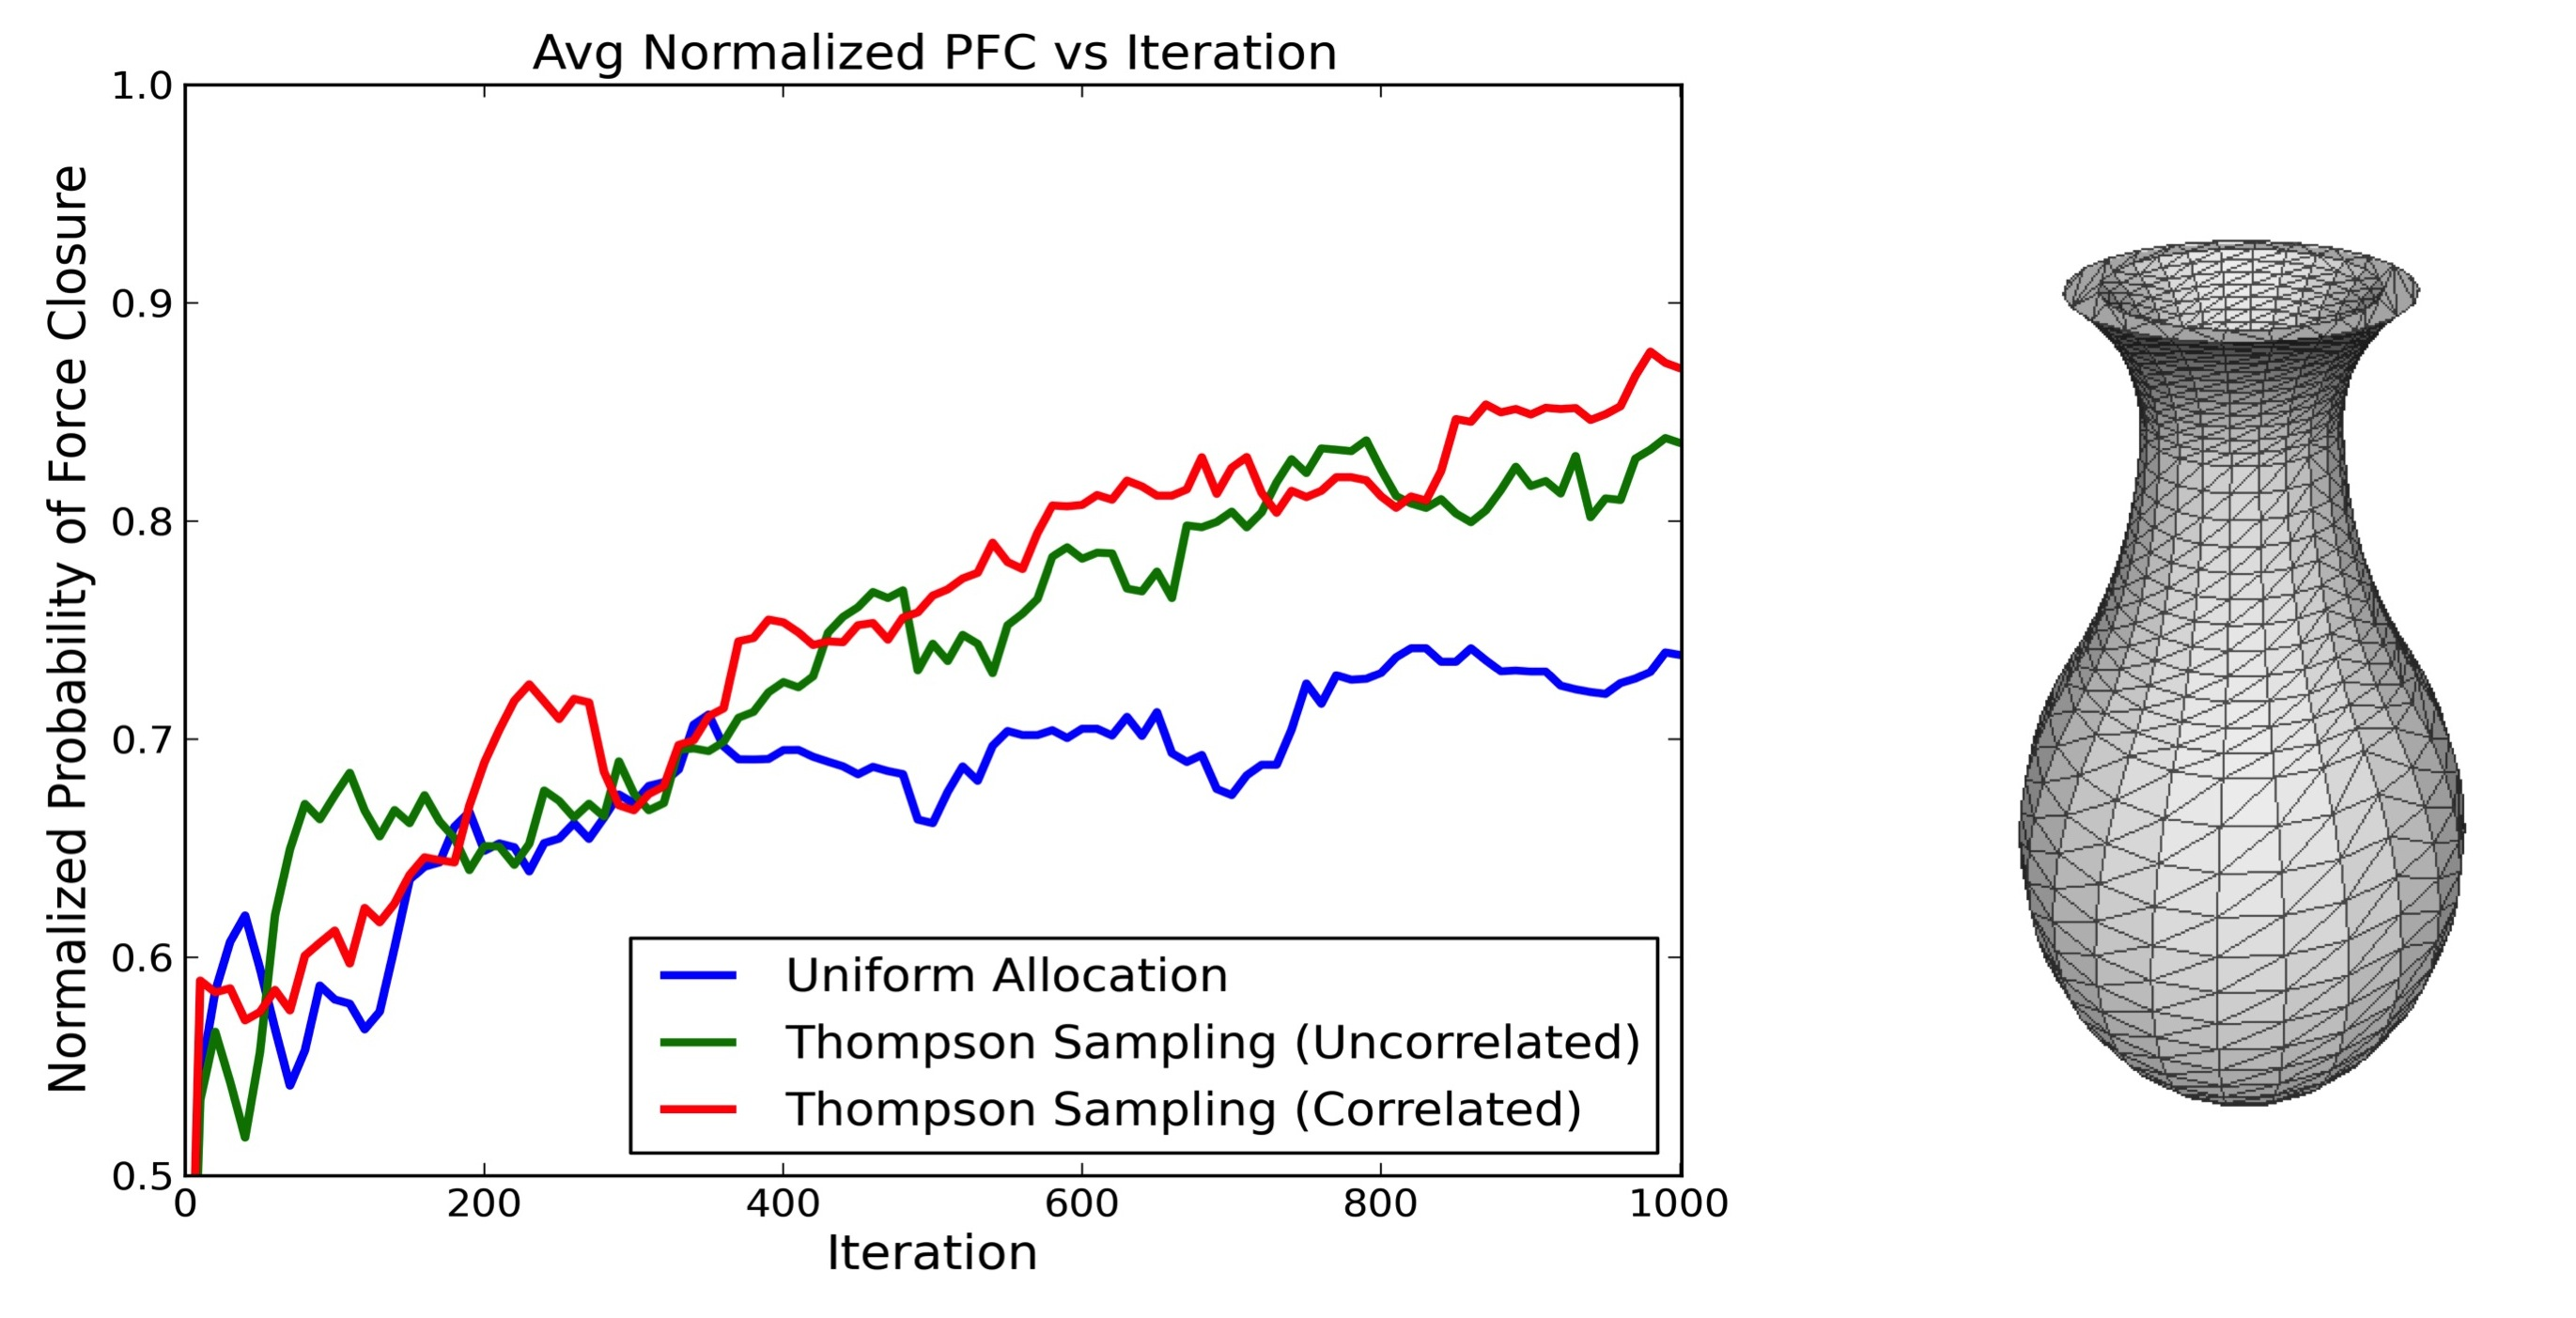
\includegraphics[scale=0.08]{figures/flowerpot_avg_reward_w_model.jpg}
        \caption{Normalized $P_F$ on a flower pot with 250 candidate grasps.}
    \end{subfigure}
\caption{Comparison of the normalized $P_F$ of the sampled grasp versus iteration of the MAB algorithm for correlated Thompson sampling, uncorrelated Thompson sampling, and Uniform Allocation averaged over 20 trials. (a) On the cereal box, correlated Thompson sampling converges to within 90\% of the highest quality grasp approximately 4$\times$ faster than uncorrelated. (b) However, correlated and uncorrelated Thompson sampling perform comparably on the flower pot because there are few grasp similarities in the candidate set. }
\figlabel{local-mab}
\vspace*{-15pt}
\end{figure}

To examine the effects of orders of magnitude of prior data in the MAB algorithms, we ran the algorithms with priors computed from increasingly larger subsets of prior data from DexNet: 0, 15, 150, and 1500 objects. 
\figref{global-mab} shows the normalized probability of force closure $P_F$ versus iteration when planning grasps for a bottle using prior grasp data from the five nearest neighbor objects in DexNet averaged over 50 trials.
Each other object was labelled with 250 grasps and $P_F$ evaluated using brute force Monte-Carlo integration.
We see that the convergence of the correlated MAB algorithms to a grasp with high $P_F$ accelerates with increasingly largers subsets of prior data used.
This suggests that adding more prior data may further accelerate convergence, because it is increasingly likely that a similar object and grasp exists in the dataset as the size increases.
Future work will examine these effects on a larger subset of objects and will use more than five nearest neighbors from DexNet to compute priors, which may lead to even larger gains for larger subsets of prior data.

\begin{figure}[t!]
\centering
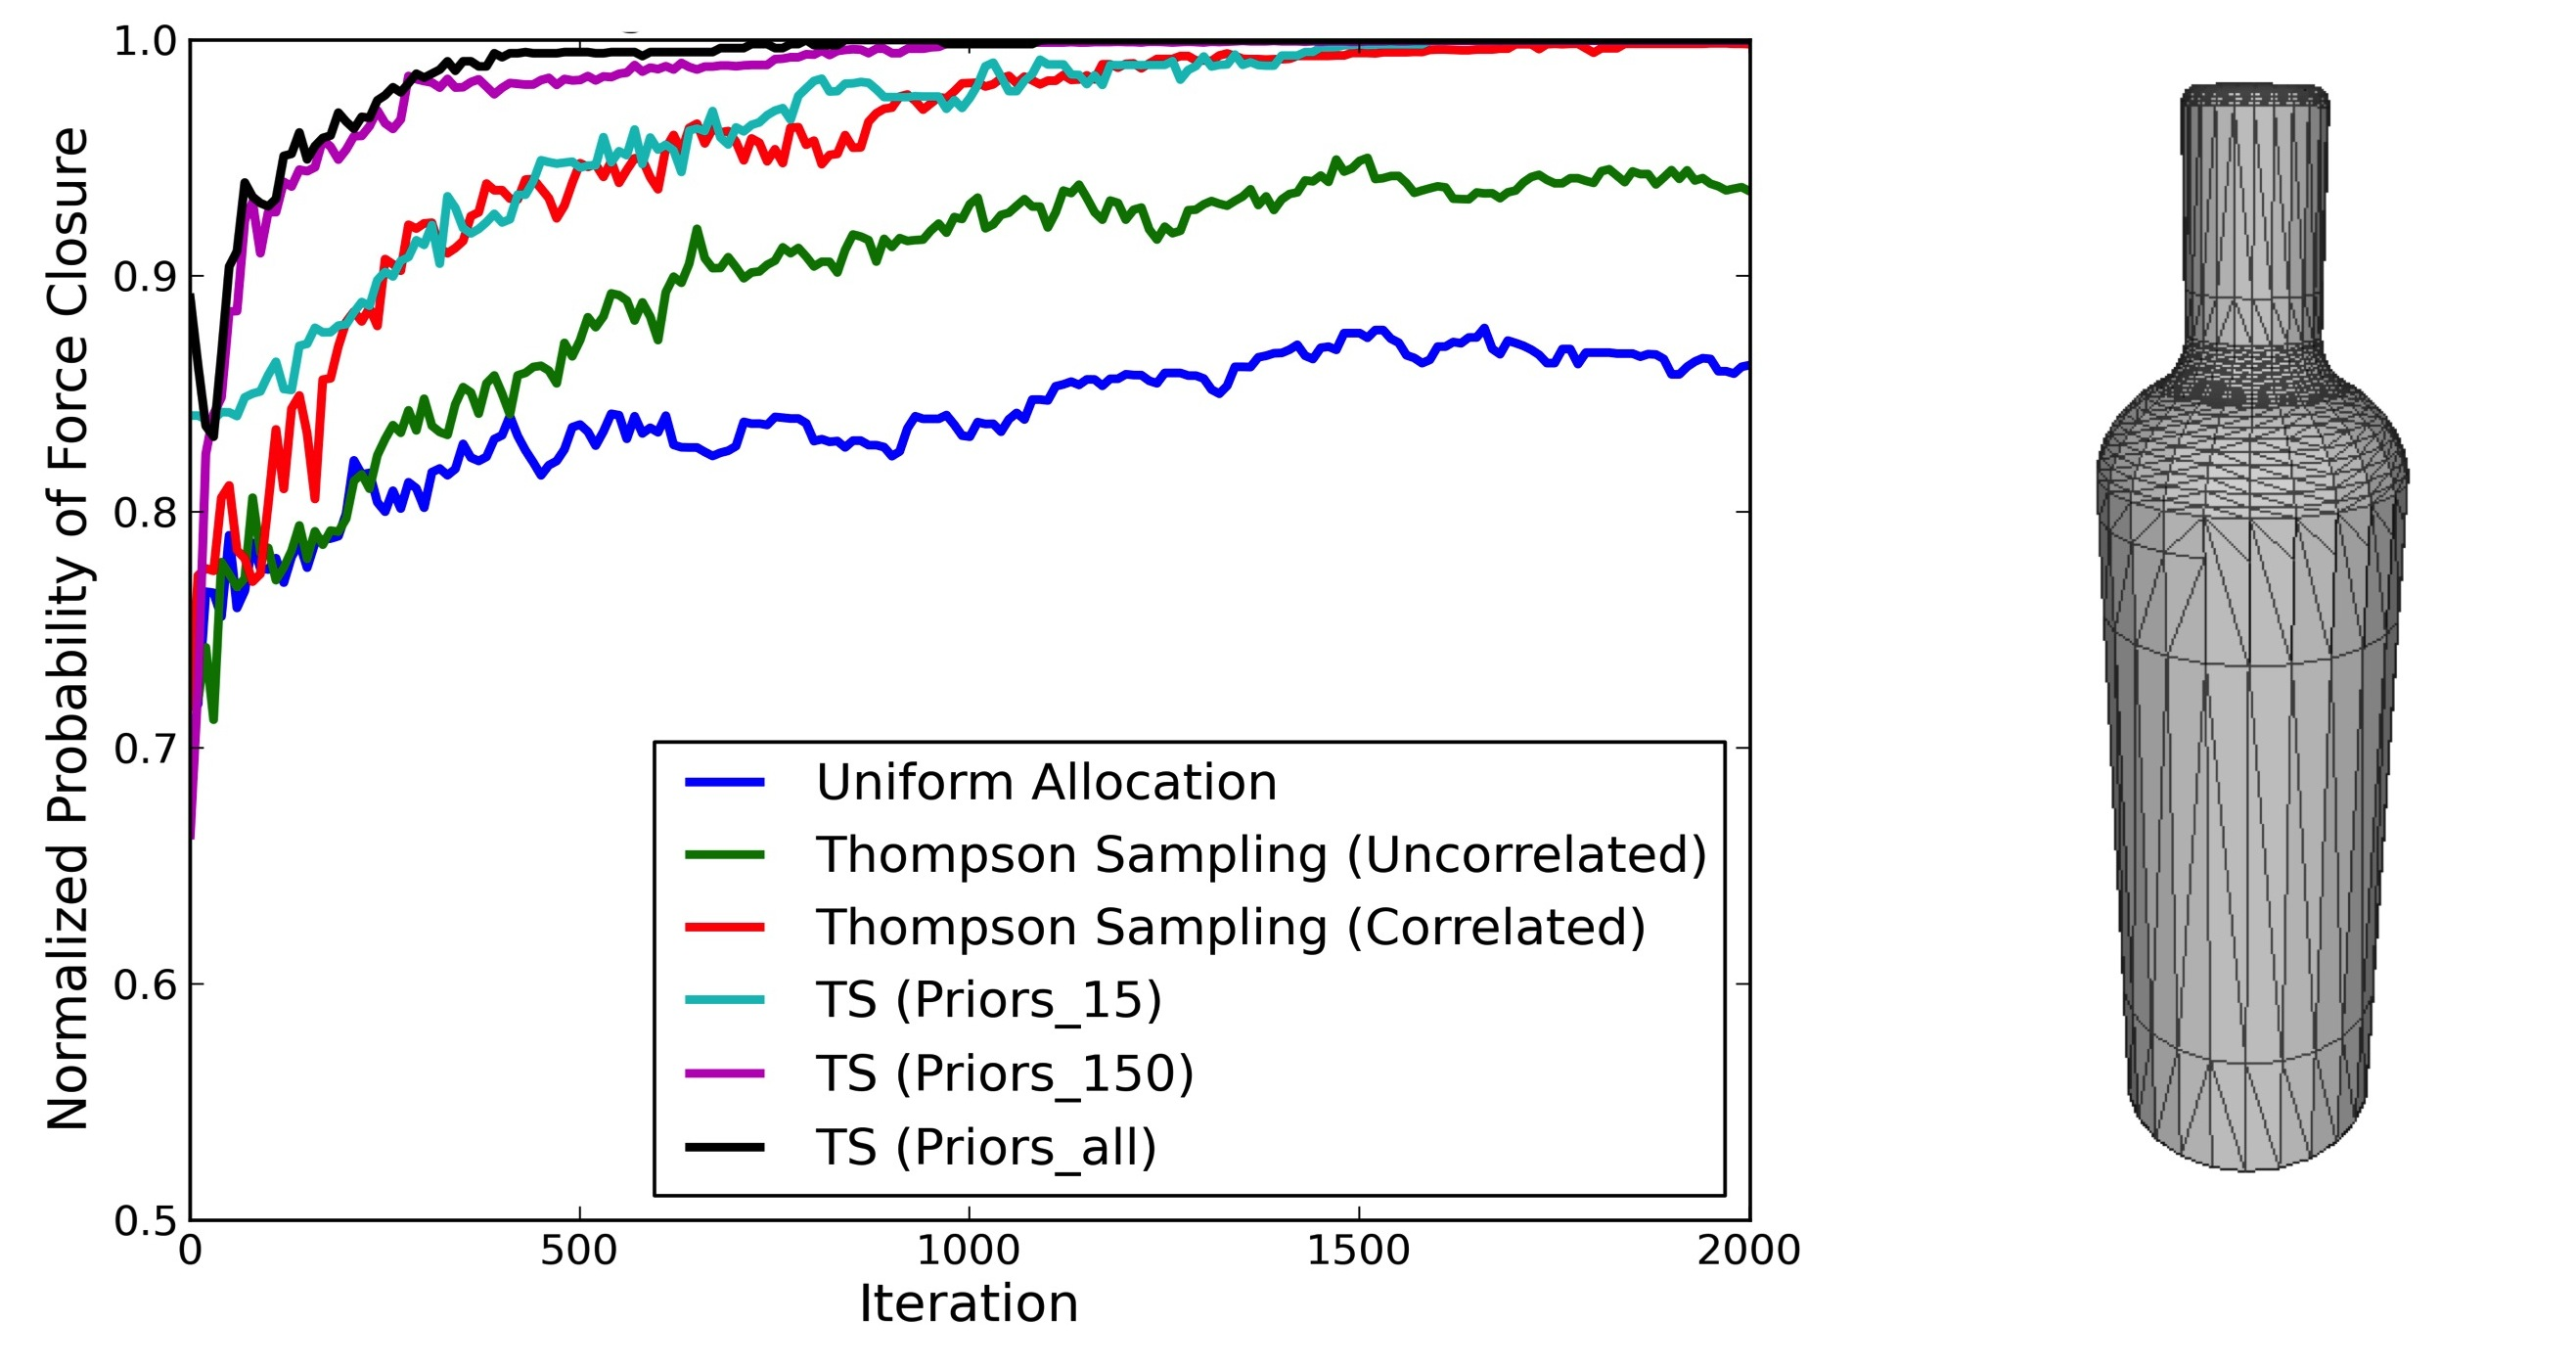
\includegraphics[scale=0.09]{figures/bottle_avg_reward_w_model2.jpg}
\caption{Comparison of the normalized $P_F$ of the sampled grasp (y-axis) versus iteration of the MAB algorithm (x-axis) for correlated Thompson sampling with and without the use of prior grasps from five nearest neighbors from DexNet, uncorrelated Thompson sampling, and Uniform Allocation averaged over 20 trials on the bottle object. Prior grasps were taken from increasingly larger subsets of DexNet: 15, 150, and 1500 objects. We see that convergence to within 90\% of the optimal grasp is accelerated by approximately 10$\times$ over uncorrelated Thompson sampling, and performance appears to improve with increasing sizes of the prior dataset used. }
\figlabel{global-mab}
\vspace*{-15pt}
\end{figure}

\TODO{Remove below section}
We are currently working on an experiment to quantify the gains in convergence time across orders of magnitudes of prior data (10, 100, 1000, 10000) from DexNet using Google Compute Engine.
Our initial version will be run on a relatively small subset of test objects, and in the coming weeks we will average the performance over a larger set of test objects.
We are particularly interested in seeing if there is a point of diminshing returns from adding more data when using datasets on the order of 10,000 - 100,000 objects.
We are also interested in whether or not adding perturbations to the data such as object reflections and shape perturbations will also increase performance, as has been observed for training Deep CNNs in vision~\cite{krizhevsky2012imagenet}.

\section{Sensitivity to Uncertainty}